\documentclass[10pt,a4paper]{article}

% Packages essentiels
\usepackage[utf8]{inputenc}
\usepackage[T1]{fontenc}
\usepackage[margin=1.5cm]{geometry}
\usepackage{amsmath,amssymb}
\usepackage{tikz}
\usetikzlibrary{positioning,calc,arrows.meta,shapes.geometric,matrix,fit}
\usepackage{xcolor}
\usepackage{listings}
\usepackage{tcolorbox}
\tcbuselibrary{breakable}
\usepackage{hyperref}
\usepackage{multicol}

% Configuration listings avec gestion complète des accents
\lstset{
    language=C,
    basicstyle=\ttfamily\scriptsize,
    backgroundcolor=\color{gray!10},
    keywordstyle=\color{blue},
    commentstyle=\color{gray},
    stringstyle=\color{red},
    numbers=left,
    numberstyle=\tiny,
    breaklines=true,
    frame=single,
    tabsize=4,
    showstringspaces=false,
    inputencoding=utf8,
    extendedchars=true,
    literate={é}{{\'e}}1 {è}{{\`e}}1 {à}{{\`a}}1 {ç}{{\c{c}}}1 
             {ê}{{\^e}}1 {î}{{\^i}}1 {ô}{{\^o}}1 {û}{{\^u}}1 {ù}{{\`u}}1
             {É}{{\'E}}1 {È}{{\`E}}1 {À}{{\`A}}1 {Ç}{{\c{C}}}1
             {Ê}{{\^E}}1 {Î}{{\^I}}1 {Ô}{{\^O}}1 {Û}{{\^U}}1 {Ù}{{\`U}}1
             {ë}{{\"e}}1 {ï}{{\"\i}}1 {ö}{{\"o}}1 {ü}{{\"u}}1
             {Ë}{{\"E}}1 {Ï}{{\"I}}1 {Ö}{{\"O}}1 {Ü}{{\"U}}1
             {œ}{{\oe}}1 {Œ}{{\OE}}1 {æ}{{\ae}}1 {Æ}{{\AE}}1
}

% Boxes pédagogiques
\newtcolorbox{definitionbox}[1]{
    colback=blue!5,colframe=blue!75!black,
    fonttitle=\bfseries,title=#1,breakable
}

\newtcolorbox{examplebox}[1]{
    colback=green!5,colframe=green!50!black,
    fonttitle=\bfseries,title=#1,breakable
}

\newtcolorbox{warningbox}[1]{
    colback=red!5,colframe=red!75!black,
    fonttitle=\bfseries,title=#1,breakable
}

\newtcolorbox{techbox}[1]{
    colback=orange!5,colframe=orange!75!black,
    fonttitle=\bfseries,title=#1,breakable
}

\newtcolorbox{infobox}[1]{
    colback=cyan!5,colframe=cyan!75!black,
    fonttitle=\bfseries,title=#1,breakable
}

\title{\textbf{Chapitre 0 : Fondamentaux du C}\\
\large Syntaxe Complète et Subtilités}
\author{Dr. El Hadji Bassirou TOURÉ\\
Département de Mathématiques et Informatique\\
Faculté des Sciences et Techniques\\
Université Cheikh Anta Diop de Dakar}
\date{}

\begin{document}

\maketitle

\section{Types et Représentation}

\subsection{Types Entiers}

Le C fournit plusieurs types entiers de tailles différentes. La taille exacte dépend de l'architecture.

\begin{techbox}{Types entiers signés}
\texttt{signed char} (au moins 8 bits), \texttt{short} (au moins 16 bits), \texttt{int} (au moins 16 bits, généralement 32), \texttt{long} (au moins 32 bits), \texttt{long long} (au moins 64 bits).
\end{techbox}

\begin{techbox}{Types entiers non signés}
Préfixe \texttt{unsigned} : \texttt{unsigned char}, \texttt{unsigned short}, \texttt{unsigned int}, \texttt{unsigned long}, \texttt{unsigned long long}.
\end{techbox}

\begin{center}
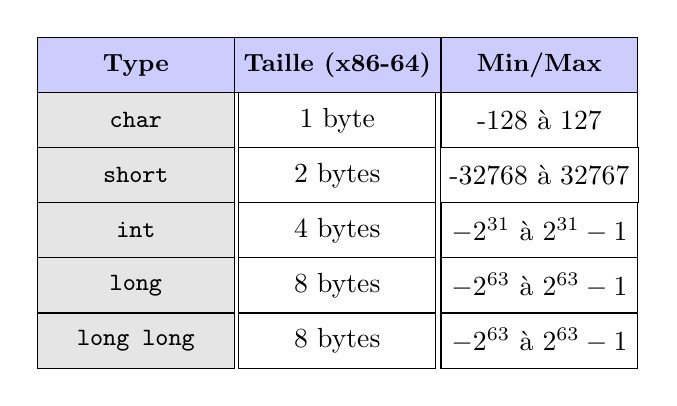
\begin{tikzpicture}[scale=0.85]
% Tableau des tailles typiques sur x86-64
\matrix (m) [matrix of nodes,
    nodes={rectangle,draw,minimum width=2.5cm,minimum height=0.7cm,anchor=center},
    column sep=-\pgflinewidth,
    row sep=-\pgflinewidth,
    nodes in empty cells,
    row 1/.style={nodes={fill=blue!20,font=\small\bfseries}},
    column 1/.style={nodes={fill=gray!20,font=\small}}
    ]
{
Type & Taille (x86-64) & Min/Max \\
\texttt{char} & 1 byte & -128 à 127 \\
\texttt{short} & 2 bytes & -32768 à 32767 \\
\texttt{int} & 4 bytes & $-2^{31}$ à $2^{31}-1$ \\
\texttt{long} & 8 bytes & $-2^{63}$ à $2^{63}-1$ \\
\texttt{long long} & 8 bytes & $-2^{63}$ à $2^{63}-1$ \\
};
\end{tikzpicture}
\end{center}

\begin{warningbox}{Garanties du standard}
Le standard C garantit uniquement : \texttt{sizeof(char)} $\leq$ \texttt{sizeof(short)} $\leq$ \texttt{sizeof(int)} $\leq$ \texttt{sizeof(long)} $\leq$ \texttt{sizeof(long long)}. Sur certaines architectures 32 bits, \texttt{long} = 4 bytes.
\end{warningbox}

\subsection{Types Flottants}

\begin{definitionbox}{Types à virgule flottante}
\texttt{float} (généralement 32 bits IEEE 754 simple précision), \texttt{double} (généralement 64 bits IEEE 754 double précision), \texttt{long double} (80 ou 128 bits selon architecture).
\end{definitionbox}

\begin{center}
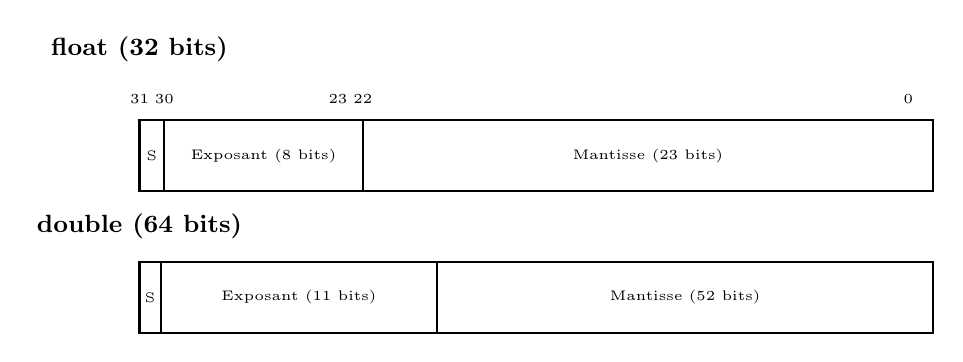
\begin{tikzpicture}[scale=0.9]
% Représentation IEEE 754 float (32 bits)
\node at (0,2) [font=\small\bfseries] {float (32 bits)};
\foreach \i/\label in {0/31,1/30,8/23,9/22,31/0} {
    \node at (\i*0.35,1.3) [font=\tiny] {\label};
}
\draw[thick] (0,0) rectangle (0.35,1);
\node at (0.175,0.5) [font=\tiny] {S};
\draw[thick] (0.35,0) rectangle (3.15,1);
\node at (1.75,0.5) [font=\tiny] {Exposant (8 bits)};
\draw[thick] (3.15,0) rectangle (11.2,1);
\node at (7.175,0.5) [font=\tiny] {Mantisse (23 bits)};

% double (64 bits) - version simplifiée
\node at (0,-0.5) [font=\small\bfseries] {double (64 bits)};
\draw[thick] (0,-2) rectangle (0.3,-1);
\node at (0.15,-1.5) [font=\tiny] {S};
\draw[thick] (0.3,-2) rectangle (4.2,-1);
\node at (2.25,-1.5) [font=\tiny] {Exposant (11 bits)};
\draw[thick] (4.2,-2) rectangle (11.2,-1);
\node at (7.7,-1.5) [font=\tiny] {Mantisse (52 bits)};
\end{tikzpicture}
\end{center}

\subsection{Type \texttt{char} et Signedness}

\begin{warningbox}{Ambiguïté du type char}
Le standard C ne spécifie PAS si \texttt{char} est signé ou non signé. Sur x86-64 (gcc), \texttt{char} est signé par défaut. Sur ARM, il est souvent non signé. Utiliser explicitement \texttt{signed char} ou \texttt{unsigned char} pour la portabilité.
\end{warningbox}

\begin{lstlisting}[caption={Comportement dépendant de l'implémentation}]
char c = 200;  // Comportement non portable
// x86-64 gcc: c = -56 (dépassement en signé)
// ARM gcc: c = 200 (non signé)

// Portable:
unsigned char uc = 200;  // Toujours 200
signed char sc = 200;    // Overflow défini: wrap around
\end{lstlisting}

\subsection{Conversions Implicites}

\begin{definitionbox}{Promotion entière}
Les types plus petits que \texttt{int} sont automatiquement promus à \texttt{int} dans les expressions. Ceci s'appelle la "promotion entière intégrale".
\end{definitionbox}

\begin{lstlisting}[caption={Promotion et conversions}]
short a = 10, b = 20;
int c = a + b;  // a et b promus en int avant addition

unsigned char uc = 255;
int i = uc + 1;  // uc promu en int, résultat = 256

// Conversion signé/non-signé (dangereux)
int si = -1;
unsigned int ui = 1;
if (si < ui)  // FAUX! si converti en unsigned: 0xFFFFFFFF > 1
    printf("si < ui\n");
else
    printf("si >= ui\n");  // S'exécute!
\end{lstlisting}

\begin{center}
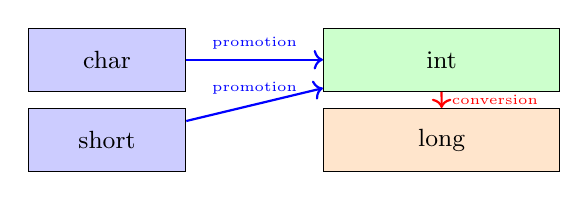
\begin{tikzpicture}[scale=0.85]
\node[rectangle,draw,fill=blue!20,minimum width=2cm,minimum height=0.8cm] (char) at (0,0) {\small char};
\node[rectangle,draw,fill=blue!20,minimum width=2cm,minimum height=0.8cm] (short) at (0,-1.2) {\small short};
\node[rectangle,draw,fill=green!20,minimum width=3cm,minimum height=0.8cm] (int) at (5,0) {\small int};
\node[rectangle,draw,fill=orange!20,minimum width=3cm,minimum height=0.8cm] (long) at (5,-1.2) {\small long};

\draw[->,thick,blue] (char) -- (int) node[midway,above,font=\tiny] {promotion};
\draw[->,thick,blue] (short) -- (int) node[midway,above,font=\tiny] {promotion};
\draw[->,thick,red] (int) -- (long) node[midway,right,font=\tiny] {conversion};
\end{tikzpicture}
\end{center}

\subsection{Opérateur \texttt{sizeof}}

\begin{definitionbox}{sizeof}
Opérateur (pas une fonction) qui retourne la taille en bytes d'un type ou d'une expression. Évalué à la compilation. Retourne un \texttt{size\_t} (entier non signé).
\end{definitionbox}

\begin{lstlisting}[caption={Utilisation de sizeof}]
// Sur des types
printf("%zu\n", sizeof(int));       // 4 (x86-64)
printf("%zu\n", sizeof(char));      // 1 (toujours)
printf("%zu\n", sizeof(double));    // 8

// Sur des variables (parenthèses optionnelles)
int x = 42;
printf("%zu\n", sizeof(x));         // 4
printf("%zu\n", sizeof x);          // 4 (valide sans parenthèses)

// Sur des expressions (non évaluées!)
int a = 5;
printf("%zu\n", sizeof(a++));       // 4, et a reste 5!
\end{lstlisting}

\begin{warningbox}{sizeof et expressions}
L'expression dans \texttt{sizeof} n'est PAS évaluée. Seul le type est déterminé à la compilation. Donc \texttt{sizeof(a++)} ne modifie pas \texttt{a}.
\end{warningbox}

\begin{lstlisting}[caption={sizeof et tableaux vs pointeurs}]
int arr[10];
int *ptr = arr;

printf("%zu\n", sizeof(arr));  // 40 (10 * 4 bytes)
printf("%zu\n", sizeof(ptr));  // 8 (taille d'un pointeur x86-64)

// Nombre d'éléments d'un tableau
size_t n = sizeof(arr) / sizeof(arr[0]);  // 10
\end{lstlisting}

\section{Variables et Classes de Stockage}

\subsection{Déclaration, Définition et Initialisation}

\begin{definitionbox}{Déclaration vs Définition}
\textbf{Déclaration} : introduit un identifiant et son type, sans allouer de mémoire.\\
\textbf{Définition} : déclaration + allocation mémoire. Toute définition est une déclaration.
\end{definitionbox}

\begin{lstlisting}[caption={Déclaration et définition de variables}]
// Définition (déclaration + allocation)
int x;              // Définition, valeur indéterminée
int y = 42;         // Définition + initialisation

// Déclaration pure (pas d'allocation ici)
extern int z;       // Déclaré ici, défini ailleurs

// Pour les fonctions
int add(int, int);  // Déclaration (prototype)
int add(int a, int b) { return a + b; }  // Définition
\end{lstlisting}

\begin{warningbox}{Variables non initialisées}
Une variable locale non initialisée a une valeur \textbf{indéterminée}. La lire est un comportement indéfini (UB). Les variables globales et \texttt{static} sont initialisées à zéro par défaut.
\end{warningbox}

\begin{lstlisting}[caption={Initialisation}]
int a;           // Global: initialisé à 0
static int b;    // Static: initialisé à 0

int main() {
    int c;       // Local: valeur INDÉTERMINÉE (UB si lu)
    int d = 0;   // Local: initialisé explicitement
    
    static int e;  // Static local: initialisé à 0
    
    printf("%d\n", c);  // UB! Valeur imprévisible
    return 0;
}
\end{lstlisting}

\subsection{Portée et Durée de Vie}

\begin{definitionbox}{Portée (scope)}
\textbf{Portée de bloc} : variable visible du point de déclaration jusqu'à la fin du bloc \texttt{\{\}}.\\
\textbf{Portée de fichier} : variable déclarée hors de toute fonction, visible dans tout le fichier.
\end{definitionbox}

\begin{lstlisting}[caption={Portée et masquage}]
int x = 10;  // Portée fichier (globale)

void foo() {
    int x = 20;  // Masque le x global
    printf("%d\n", x);  // 20
    
    {
        int x = 30;  // Masque le x de foo
        printf("%d\n", x);  // 30
    }
    
    printf("%d\n", x);  // 20 (x de foo)
}

int main() {
    printf("%d\n", x);  // 10 (x global)
    foo();
    return 0;
}
\end{lstlisting}

\begin{techbox}{Durée de vie}
\textbf{Automatique} : durée du bloc (variables locales).\\
\textbf{Statique} : durée du programme (globales et \texttt{static}).
\end{techbox}

\subsection{Classes de Stockage}

\begin{definitionbox}{auto (implicite)}
Classe par défaut pour les variables locales. Allocation sur la pile, durée de vie = bloc englobant.
\end{definitionbox}

\begin{lstlisting}[caption={auto (rarement écrit explicitement)}]
void foo() {
    auto int x = 5;  // Équivalent à: int x = 5;
    // auto est implicite pour les locales
}
\end{lstlisting}

\begin{definitionbox}{static}
\textbf{Variable locale static} : durée de vie = programme, portée = bloc.\\
\textbf{Variable globale static} : portée limitée au fichier (liaison interne).\\
\textbf{Fonction static} : visible uniquement dans le fichier.
\end{definitionbox}

\begin{lstlisting}[caption={static local : persistance entre appels}]
void counter() {
    static int count = 0;  // Initialisé UNE seule fois
    count++;
    printf("Appel #%d\n", count);
}

int main() {
    counter();  // Appel #1
    counter();  // Appel #2
    counter();  // Appel #3
    return 0;
}
\end{lstlisting}

\begin{lstlisting}[caption={static global : encapsulation au fichier}]
// fichier: module.c
static int internal_counter = 0;  // Invisible hors de ce fichier
static void helper() { }          // Fonction interne

void public_api() {  // Visible partout
    internal_counter++;
    helper();
}
\end{lstlisting}

\begin{definitionbox}{extern}
Déclare une variable ou fonction définie dans un autre fichier (liaison externe). Pas d'allocation, juste une référence.
\end{definitionbox}

\begin{lstlisting}[caption={extern : exemple multi-fichiers}]
// === config.h ===
#ifndef CONFIG_H
#define CONFIG_H
extern int global_count;    // Déclaration
extern void increment();    // Déclaration (extern implicite)
#endif

// === config.c ===
#include "config.h"
int global_count = 0;       // Définition (une seule fois)

void increment() {          // Définition
    global_count++;
}

// === main.c ===
#include <stdio.h>
#include "config.h"

int main() {
    printf("%d\n", global_count);  // 0
    increment();
    increment();
    printf("%d\n", global_count);  // 2
    return 0;
}

// Compilation: gcc -o prog main.c config.c
\end{lstlisting}

\begin{warningbox}{Erreurs courantes avec extern}
\begin{itemize}
\item Oublier la définition : erreur de linkage "undefined reference"
\item Définir plusieurs fois : erreur "multiple definition"
\item Initialiser dans la déclaration extern : devient une définition!
\end{itemize}
\end{warningbox}

\begin{lstlisting}[caption={Erreurs avec extern}]
// ERREUR: extern avec initialisation = définition
extern int x = 5;  // C'est une DÉFINITION, pas une déclaration

// CORRECT
extern int x;      // Déclaration
int x = 5;         // Définition (dans un autre fichier ou plus bas)
\end{lstlisting}

\subsection{Constantes : \texttt{const} vs \texttt{\#define}}

\begin{techbox}{const}
Qualificateur de type. La variable est en lecture seule après initialisation. Typée, scopée, visible au débogueur.
\end{techbox}

\begin{techbox}{\#define}
Directive préprocesseur. Substitution textuelle avant compilation. Pas de type, portée = fin du fichier (ou \texttt{\#undef}).
\end{techbox}

\begin{lstlisting}[caption={const vs \#define}]
#define MAX_MACRO 100       // Substitution textuelle
const int MAX_CONST = 100;  // Variable constante

// Typage
#define PI_MACRO 3.14159
const double PI_CONST = 3.14159;

// Scope
void foo() {
    #define LOCAL_MACRO 42  // Visible PARTOUT après cette ligne!
    const int LOCAL_CONST = 42;  // Visible seulement dans foo
}

// Débogage
// gdb peut afficher MAX_CONST, pas MAX_MACRO (disparu après préprocesseur)
\end{lstlisting}

\begin{lstlisting}[caption={Pièges du \#define}]
#define SQUARE(x) x * x

int a = SQUARE(3);      // 3 * 3 = 9, OK
int b = SQUARE(1 + 2);  // 1 + 2 * 1 + 2 = 5, FAUX!

// Solution: parenthèses
#define SQUARE_SAFE(x) ((x) * (x))
int c = SQUARE_SAFE(1 + 2);  // ((1 + 2) * (1 + 2)) = 9, OK

// Mais toujours des problèmes
int d = SQUARE_SAFE(a++);  // ((a++) * (a++)) : a incrémenté 2 fois!
\end{lstlisting}

\begin{warningbox}{Recommandation}
Préférer \texttt{const} à \texttt{\#define} pour les constantes. Utiliser \texttt{\#define} pour la compilation conditionnelle et les macros complexes uniquement.
\end{warningbox}

\section{Opérateurs et Évaluation}

\subsection{Opérateurs Arithmétiques}

\begin{techbox}{Opérateurs arithmétiques}
\texttt{+}, \texttt{-}, \texttt{*}, \texttt{/}, \texttt{\%} (modulo, entiers seulement).\\
Division entière : \texttt{7 / 2 = 3}, \texttt{-7 / 2 = -3} (troncature vers zéro en C99).\\
Modulo : signe du résultat = signe du dividende.
\end{techbox}

\begin{lstlisting}[caption={Division et modulo}]
int a = 7 / 2;      // 3
int b = -7 / 2;     // -3 (C99: troncature vers zéro)
int c = 7 % 2;      // 1
int d = -7 % 2;     // -1 (signe de -7)
int e = 7 % -2;     // 1 (signe de 7)

// Attention au type!
float f = 7 / 2;    // 3.0 (division entière puis conversion)
float g = 7.0 / 2;  // 3.5 (division flottante)
\end{lstlisting}

\subsection{Opérateurs Bit à Bit}

\begin{techbox}{Opérateurs bit à bit (entiers seulement)}
\texttt{\&} (AND), \texttt{|} (OR), \texttt{\^{}} (XOR), \texttt{\~{}} (NOT), \texttt{<<} (shift gauche), \texttt{>>} (shift droite).
\end{techbox}

\begin{lstlisting}[caption={Opérations bit à bit}]
unsigned int x = 0x89AB;  // 1000 1001 1010 1011
unsigned int y = 0x1234;  // 0001 0010 0011 0100

unsigned int a = x & y;   // 0x0020 (AND)
unsigned int b = x | y;   // 0x9BBF (OR)
unsigned int c = x ^ y;   // 0x9B9F (XOR)
unsigned int d = ~x;      // 0xFFFF7654 (NOT, 32 bits)

// Shifts
unsigned int e = x << 2;  // 0x226AC (shift gauche, * 4)
unsigned int f = x >> 2;  // 0x226A (shift droite logique, / 4)

// Shift droite signé vs non-signé
int si = -8;              // 0xFFFFFFF8
int g = si >> 1;          // -4 (shift arithmétique: sign extend)
unsigned int ui = -8;
unsigned int h = ui >> 1; // 0x7FFFFFFC (shift logique: zéro extend)
\end{lstlisting}

\begin{warningbox}{Shift droite et type signé}
Le comportement de \texttt{>>} sur les types signés est défini par l'implémentation (généralement arithmétique avec extension de signe). Utiliser des types non signés pour des manipulations de bits prévisibles.
\end{warningbox}

\subsection{Opérateurs Logiques et Court-Circuit}

\begin{definitionbox}{Opérateurs logiques}
\texttt{\&\&} (AND logique), \texttt{||} (OR logique), \texttt{!} (NOT logique). Évaluation en court-circuit : \texttt{\&\&} s'arrête au premier faux, \texttt{||} au premier vrai.
\end{definitionbox}

\begin{lstlisting}[caption={Court-circuit et side-effects}]
int a = 0, b = 0;

// && court-circuite
if (a != 0 && b/a > 2) {  // b/a non évalué car a == 0
    printf("OK\n");
}

// Ordre d'évaluation garanti
int c = 0;
if (++c > 0 && ++c > 1) {  // c = 2 après évaluation
    printf("c = %d\n", c);
}

// Erreur classique: & au lieu de &&
if (a != 0 & b/a > 2) {  // ERREUR: & évalue les deux côtés!
    printf("Crash si a == 0\n");
}
\end{lstlisting}

\subsection{Opérateurs d'Incrémentation}

\begin{techbox}{Incrémentation et décrémentation}
\texttt{++x} (pré-incrémentation : incrémente puis retourne), \texttt{x++} (post-incrémentation : retourne puis incrémente). Idem pour \texttt{-{}-}.
\end{techbox}

\begin{lstlisting}[caption={Pré vs post incrémentation}]
int a = 5, b, c;

b = ++a;  // a = 6, b = 6 (pré-incrémentation)
c = a++;  // c = 6, a = 7 (post-incrémentation)

// Danger: modification multiple dans une expression
int x = 5;
int y = (x++) + (++x);  // COMPORTEMENT INDÉFINI (UB)!
// x modifié deux fois sans sequence point
\end{lstlisting}

\subsection{Opérateur Ternaire}

\begin{definitionbox}{Opérateur ternaire}
\texttt{condition ? valeur\_si\_vrai : valeur\_si\_faux}. Seule l'expression sélectionnée est évaluée.
\end{definitionbox}

\begin{lstlisting}[caption={Ternaire et side-effects}]
int a = 10, b = 20;
int max = (a > b) ? a : b;  // max = 20

// Side-effect dans une seule branche
int c = 0;
int d = (a > b) ? ++c : ++a;  // Seulement ++a exécuté
// c = 0, a = 11, d = 11
\end{lstlisting}

\subsection{Précédence et Associativité}

\begin{center}
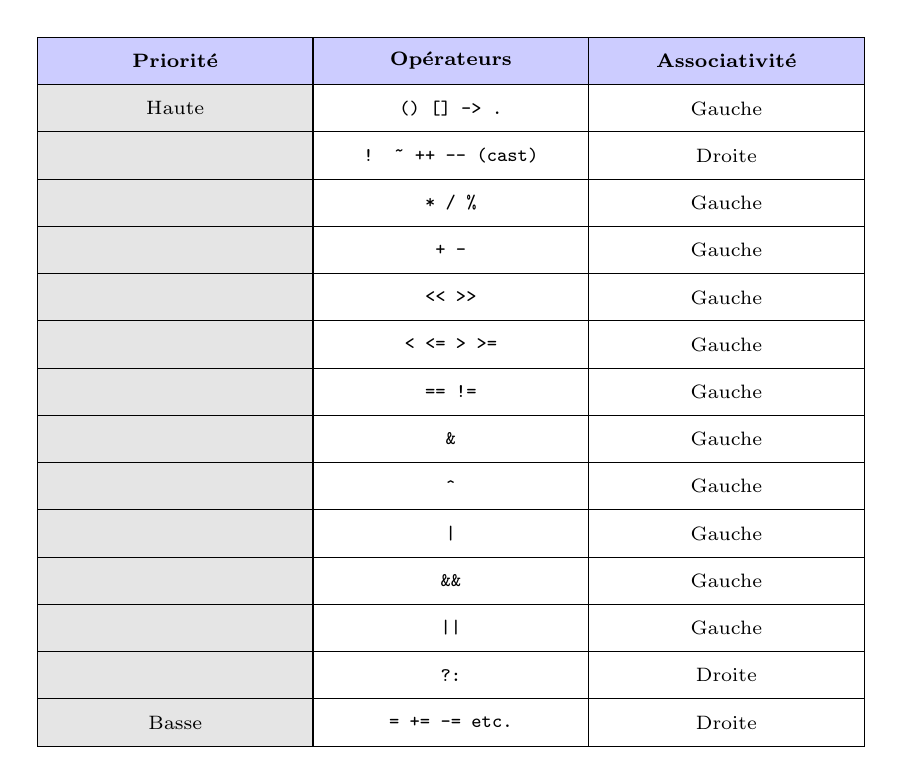
\begin{tikzpicture}[scale=0.75]
\matrix (m) [matrix of nodes,
    nodes={rectangle,draw,minimum width=3.5cm,minimum height=0.6cm,anchor=center,font=\scriptsize},
    column sep=-\pgflinewidth,
    row sep=-\pgflinewidth,
    nodes in empty cells,
    row 1/.style={nodes={fill=blue!20,font=\scriptsize\bfseries}},
    column 1/.style={nodes={fill=gray!20}}
    ]
{
Priorité & Opérateurs & Associativité \\
Haute & \texttt{() [] -> .} & Gauche \\
& \texttt{! \~{} ++ -{}- (cast)} & Droite \\
& \texttt{* / \%} & Gauche \\
& \texttt{+ -} & Gauche \\
& \texttt{<< >>} & Gauche \\
& \texttt{< <= > >=} & Gauche \\
& \texttt{== !=} & Gauche \\
& \texttt{\&} & Gauche \\
& \texttt{\^{}} & Gauche \\
& \texttt{|} & Gauche \\
& \texttt{\&\&} & Gauche \\
& \texttt{||} & Gauche \\
& \texttt{?:} & Droite \\
Basse & \texttt{= += -= etc.} & Droite \\
};
\end{tikzpicture}
\end{center}

\begin{lstlisting}[caption={Pièges de précédence}]
int a = 5, b = 10, c;

// Priorité inattendue
c = a & b == 5;  // Équivalent à: a & (b == 5)
// NON (a & b) == 5 !

// Shift et addition
c = 1 << 2 + 3;  // Équivalent à: 1 << (2 + 3) = 32
// NON (1 << 2) + 3 = 7 !
\end{lstlisting}

\section{Structures de Contrôle}

\subsection{Conditionnelle \texttt{if-else}}

\begin{definitionbox}{Syntaxe if-else}
\texttt{if (condition) instruction;} ou \texttt{if (condition) \{...\} else \{...\}}. La condition est vraie si non nulle.
\end{definitionbox}

\begin{lstlisting}[caption={If-else et dangling else}]
int a = 10, b = 20, c = 30;

// Bloc simple
if (a > b)
    printf("a > b\n");

// Dangling else (associé au if le plus proche)
if (a > 5)
    if (b > 15)
        printf("Les deux\n");
    else  // Ce else est associé au deuxième if!
        printf("Seulement b <= 15\n");

// Solution: accolades explicites
if (a > 5) {
    if (b > 15)
        printf("Les deux\n");
} else {
    printf("a <= 5\n");
}
\end{lstlisting}

\subsection{Conditionnelle \texttt{switch}}

\begin{definitionbox}{Syntaxe switch}
\texttt{switch (expression) \{ case constante: ... break; default: ... \}}. L'expression doit être de type entier. Le \texttt{break} est nécessaire pour éviter le fall-through.
\end{definitionbox}

\begin{lstlisting}[caption={Switch et fall-through}]
int day = 3;

switch (day) {
    case 1:
        printf("Lundi\n");
        break;
    case 2:
        printf("Mardi\n");
        break;
    case 3:
        printf("Mercredi\n");
        // OUBLI de break: fall-through!
    case 4:
        printf("Jeudi\n");  // Exécuté aussi!
        break;
    default:
        printf("Autre jour\n");
}

// Fall-through intentionnel
switch (day) {
    case 1: case 2: case 3: case 4: case 5:
        printf("Jour de semaine\n");
        break;
    case 6: case 7:
        printf("Weekend\n");
        break;
}
\end{lstlisting}

\begin{warningbox}{Limites du switch}
Les étiquettes \texttt{case} doivent être des constantes de compilation. Pas de \texttt{case x:} si \texttt{x} est une variable. Pas de \texttt{case 1...5:} (extension gcc).
\end{warningbox}

\subsection{Boucle \texttt{while}}

\begin{definitionbox}{Syntaxe while}
\texttt{while (condition) instruction;}. La condition est évaluée AVANT chaque itération. Si fausse initialement, le corps ne s'exécute jamais.
\end{definitionbox}

\begin{lstlisting}[caption={While et condition}]
int i = 0;
while (i < 10) {
    printf("%d ", i);
    i++;
}  // Affiche: 0 1 2 3 4 5 6 7 8 9

// Boucle infinie
while (1) {
    // ...
    if (condition)
        break;  // Sortie de la boucle
}
\end{lstlisting}

\subsection{Boucle \texttt{do-while}}

\begin{definitionbox}{Syntaxe do-while}
\texttt{do instruction; while (condition);}. La condition est évaluée APRÈS chaque itération. Le corps s'exécute au moins une fois.
\end{definitionbox}

\begin{lstlisting}[caption={Do-while et exécution garantie}]
int i = 10;

// while: ne s'exécute pas
while (i < 10) {
    printf("while: %d\n", i);
}

// do-while: s'exécute une fois
do {
    printf("do-while: %d\n", i);  // Affiche une fois
} while (i < 10);
\end{lstlisting}

\subsection{Boucle \texttt{for}}

\begin{definitionbox}{Syntaxe for}
\texttt{for (initialisation; condition; incrémentation) instruction;}. Équivalent à un \texttt{while} avec initialisation et incrémentation intégrées.
\end{definitionbox}

\begin{lstlisting}[caption={For et équivalence}]
// Forme classique
for (int i = 0; i < 10; i++) {
    printf("%d ", i);
}

// Équivalent while
{
    int i = 0;
    while (i < 10) {
        printf("%d ", i);
        i++;
    }
}

// Sections optionnelles
int i = 0;
for (; i < 10; ) {  // Init et incr omises
    printf("%d ", i);
    i++;
}

// Boucle infinie
for (;;) {  // Toutes sections omises
    // ...
}
\end{lstlisting}

\subsection{Instructions \texttt{break} et \texttt{continue}}

\begin{techbox}{Break et continue}
\texttt{break} : sort de la boucle ou du \texttt{switch} englobant.\\
\texttt{continue} : passe à l'itération suivante de la boucle englobante.
\end{techbox}

\begin{lstlisting}[caption={Break et continue}]
// Break: sortie de boucle
for (int i = 0; i < 10; i++) {
    if (i == 5)
        break;  // Sort de la boucle
    printf("%d ", i);
}  // Affiche: 0 1 2 3 4

// Continue: itération suivante
for (int i = 0; i < 10; i++) {
    if (i % 2 == 0)
        continue;  // Passe aux nombres impairs
    printf("%d ", i);
}  // Affiche: 1 3 5 7 9

// Boucles imbriquées: break sort de la boucle IMMÉDIATE
for (int i = 0; i < 3; i++) {
    for (int j = 0; j < 3; j++) {
        if (j == 1)
            break;  // Sort de la boucle j, pas i
        printf("(%d,%d) ", i, j);
    }
}  // Affiche: (0,0) (1,0) (2,0)
\end{lstlisting}

\subsection{Instruction \texttt{goto}}

\begin{definitionbox}{Syntaxe goto}
\texttt{goto étiquette;} suivi de \texttt{étiquette:} ailleurs dans la même fonction. Saut inconditionnel vers l'étiquette.
\end{definitionbox}

\begin{warningbox}{Usage de goto (Dijkstra, 1968)}
Edsger W. Dijkstra, dans son article "Go To Statement Considered Harmful" (1968), a démontré que \texttt{goto} rend le code difficile à comprendre et à maintenir. L'utilisation de \texttt{goto} est généralement déconseillée en programmation moderne.

\textbf{Cas acceptables (rares):}
\begin{itemize}
\item Sortie de boucles profondément imbriquées
\item Gestion d'erreurs avec nettoyage (pattern Linux kernel)
\end{itemize}

\textbf{À éviter absolument:}
\begin{itemize}
\item Sauts en arrière créant des boucles (utiliser \texttt{while}, \texttt{for})
\item Sauts complexes rendant le flux de contrôle illisible
\end{itemize}
\end{warningbox}

\begin{lstlisting}[caption={Goto: sortie de boucles imbriquées}]
// Problème: break ne sort que d'une boucle
int found = 0;
for (int i = 0; i < 10 && !found; i++) {
    for (int j = 0; j < 10; j++) {
        if (condition(i, j)) {
            found = 1;
            break;  // Sort seulement de la boucle j
        }
    }
}

// Solution avec goto (acceptable)
for (int i = 0; i < 10; i++) {
    for (int j = 0; j < 10; j++) {
        if (condition(i, j)) {
            goto found;  // Sort des deux boucles
        }
    }
}
found:
printf("Trouvé\n");
\end{lstlisting}

\begin{lstlisting}[caption={Goto: gestion d'erreurs (pattern kernel)}]
int process_data(void) {
    int *buffer1 = malloc_int();
    if (buffer1 == NULL)
        goto error_buffer1;
    
    int *buffer2 = malloc_int();
    if (buffer2 == NULL)
        goto error_buffer2;
    
    int *buffer3 = malloc_int();
    if (buffer3 == NULL)
        goto error_buffer3;
    
    // Traitement normal
    process(buffer1, buffer2, buffer3);
    
    // Nettoyage normal
    free_int(buffer3);
error_buffer3:
    free_int(buffer2);
error_buffer2:
    free_int(buffer1);
error_buffer1:
    return -1;  // Ou code d'erreur approprié
}
\end{lstlisting}

\begin{lstlisting}[caption={Transformation goto → boucles structurées}]
// Avec goto (à éviter: boucle déguisée)
int i = 0;
loop_start:
    printf("%d ", i);
    i++;
    if (i < 10)
        goto loop_start;

// Sans goto (préférable)
for (int i = 0; i < 10; i++) {
    printf("%d ", i);
}

// Avec goto (acceptable: sortie multiple)
for (int i = 0; i < 100; i++) {
    for (int j = 0; j < 100; j++) {
        if (i * j > 500)
            goto end;  // Sortie propre
    }
}
end:
printf("Terminé\n");

// Sans goto (avec flag, moins lisible)
int done = 0;
for (int i = 0; i < 100 && !done; i++) {
    for (int j = 0; j < 100; j++) {
        if (i * j > 500) {
            done = 1;
            break;
        }
    }
}
printf("Terminé\n");
\end{lstlisting}

\begin{lstlisting}[caption={Anti-patterns avec goto}]
// MAUVAIS: goto en arrière créant une boucle
int i = 0;
start:
    printf("%d ", i);
    i++;
    if (i < 10)
        goto start;  // Utiliser for/while à la place!

// MAUVAIS: sauts croisés illisibles
if (condition1)
    goto label2;
// code
label1:
    // code
    if (condition2)
        goto label3;
label2:
    // code
    goto label1;
label3:
    // Spaghetti code!

// MAUVAIS: saut dans un bloc
if (condition) {
    // code
label:  // Sauter ici depuis l'extérieur est dangereux
    // code
}
goto label;  // Variables locales non initialisées!
\end{lstlisting}

\section{Fonctions}

\subsection{Déclaration et Définition}

\begin{definitionbox}{Déclaration vs définition}
\textbf{Déclaration} : prototype de fonction (signature uniquement).\\
\textbf{Définition} : implémentation complète de la fonction.
\end{definitionbox}

\begin{lstlisting}[caption={Déclaration et définition}]
// Déclaration (prototype)
int add(int a, int b);  // Noms des paramètres optionnels

// Définition
int add(int a, int b) {
    return a + b;
}

// Déclaration sans prototype (K&R style, obsolète)
int multiply();  // Pas d'info sur les paramètres

// Appel
int x = add(5, 10);
\end{lstlisting}

\subsection{Passage par Valeur}

\begin{techbox}{Passage par valeur}
En C, les arguments sont TOUJOURS passés par valeur. Une copie de la valeur est transmise à la fonction. Modifications locales n'affectent pas l'appelant.
\end{techbox}

\begin{lstlisting}[caption={Passage par valeur}]
void increment(int x) {
    x++;  // Modifie la copie locale
}

int main() {
    int a = 5;
    increment(a);
    printf("%d\n", a);  // Affiche: 5 (inchangé)
    return 0;
}

// Pour modifier: passer l'adresse (pointeur)
void increment_ptr(int *x) {
    (*x)++;
}

int main() {
    int a = 5;
    increment_ptr(&a);
    printf("%d\n", a);  // Affiche: 6
    return 0;
}
\end{lstlisting}

\subsection{Valeur de Retour}

\begin{techbox}{Return}
\texttt{return expression;} termine la fonction et retourne une valeur. Type de retour doit correspondre à la déclaration. \texttt{return;} pour fonctions \texttt{void}.
\end{techbox}

\begin{lstlisting}[caption={Valeurs de retour}]
int max(int a, int b) {
    if (a > b)
        return a;
    return b;  // Un seul return possible par exécution
}

// Fonction void
void print_max(int a, int b) {
    printf("Max: %d\n", max(a, b));
    return;  // Optionnel pour void
}

// Return dans boucle
int find_first_positive(int arr[], int size) {
    for (int i = 0; i < size; i++) {
        if (arr[i] > 0)
            return i;  // Retour immédiat
    }
    return -1;  // Non trouvé
}
\end{lstlisting}

\subsection{Fonctions Récursives}

\begin{definitionbox}{Récursion}
Une fonction peut s'appeler elle-même. Nécessite un cas de base pour éviter la récursion infinie. La pile d'appels stocke les contextes d'exécution.
\end{definitionbox}

\begin{lstlisting}[caption={Fonction récursive}]
// Factorielle
int factorial(int n) {
    if (n <= 1)  // Cas de base
        return 1;
    return n * factorial(n - 1);  // Appel récursif
}

// Fibonacci
int fibonacci(int n) {
    if (n <= 1)
        return n;
    return fibonacci(n - 1) + fibonacci(n - 2);
}

// Danger: récursion infinie
int infinite(int n) {
    return infinite(n);  // Stack overflow!
}
\end{lstlisting}

\section{Compilation}

\subsection{Phases de Compilation}

\begin{center}
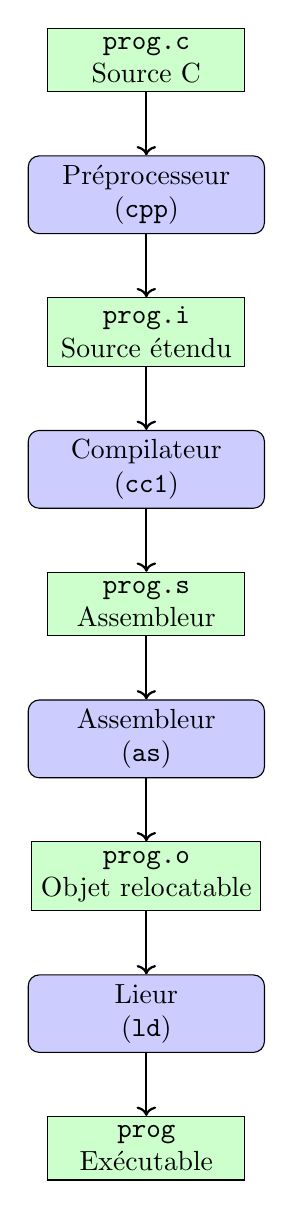
\begin{tikzpicture}[scale=0.85,
    phase/.style={rectangle,rounded corners,draw,fill=blue!20,minimum width=3cm,minimum height=0.9cm,align=center},
    file/.style={rectangle,draw,fill=green!20,minimum width=2.5cm,minimum height=0.7cm,align=center},
    node distance=0.8cm]

\node[file] (source) at (0,0) {\texttt{prog.c}\\Source C};
\node[phase] (cpp) [below=of source] {Préprocesseur\\(\texttt{cpp})};
\node[file] (i) [below=of cpp] {\texttt{prog.i}\\Source étendu};
\node[phase] (cc1) [below=of i] {Compilateur\\(\texttt{cc1})};
\node[file] (s) [below=of cc1] {\texttt{prog.s}\\Assembleur};
\node[phase] (as) [below=of s] {Assembleur\\(\texttt{as})};
\node[file] (o) [below=of as] {\texttt{prog.o}\\Objet relocatable};
\node[phase] (ld) [below=of o] {Lieur\\(\texttt{ld})};
\node[file] (exe) [below=of ld] {\texttt{prog}\\Exécutable};

\draw[->,thick] (source) -- (cpp);
\draw[->,thick] (cpp) -- (i);
\draw[->,thick] (i) -- (cc1);
\draw[->,thick] (cc1) -- (s);
\draw[->,thick] (s) -- (as);
\draw[->,thick] (as) -- (o);
\draw[->,thick] (o) -- (ld);
\draw[->,thick] (ld) -- (exe);
\end{tikzpicture}
\end{center}

\subsection{Préprocesseur}

\begin{techbox}{Directives du préprocesseur}
\texttt{\#include}, \texttt{\#define}, \texttt{\#ifdef}, \texttt{\#ifndef}, \texttt{\#endif}, \texttt{\#if}, \texttt{\#else}, \texttt{\#elif}. Traitement textuel avant compilation.
\end{techbox}

\begin{lstlisting}[caption={Préprocesseur}]
#include <stdio.h>  // Inclusion de header standard
#include "myheader.h"  // Inclusion de header local

#define MAX 100  // Macro constante
#define SQUARE(x) ((x) * (x))  // Macro fonction

// Compilation conditionnelle
#ifdef DEBUG
    printf("Debug mode\n");
#endif

// Afficher le résultat du préprocesseur
// gcc -E prog.c -o prog.i
\end{lstlisting}

\subsection{Options de Compilation}

\begin{techbox}{Options gcc importantes}
\texttt{-Wall} (warnings), \texttt{-Wextra}, \texttt{-Werror}, \texttt{-std=c99}, \texttt{-O0/-O1/-O2/-O3} (optimisation), \texttt{-g} (debug), \texttt{-S} (assembleur), \texttt{-c} (objet).
\end{techbox}

\begin{lstlisting}[language=bash,caption={Commandes gcc}]
# Compilation complète
gcc -Wall -Wextra -O2 -o prog prog.c

# Compilation séparée
gcc -c -Wall file1.c  # Génère file1.o
gcc -c -Wall file2.c  # Génère file2.o
gcc -o prog file1.o file2.o  # Linkage

# Voir l'assembleur
gcc -S -O0 prog.c  # Génère prog.s

# Debug avec gdb
gcc -g -o prog prog.c
gdb prog
\end{lstlisting}

\section{Comportement Indéfini (UB)}

\subsection{Définition}

\begin{warningbox}{Undefined Behavior}
Comportement indéfini (UB) : le standard C ne spécifie PAS ce qui se passe. Le compilateur peut faire n'importe quoi : crash, résultat inattendu, code optimisé incorrectement, démons nasaux.
\end{warningbox}

\subsection{Exemples Classiques}

\begin{lstlisting}[caption={UB courants}]
// 1. Division par zéro
int a = 5 / 0;  // UB

// 2. Dépassement d'entier signé
int x = INT_MAX + 1;  // UB (entiers signés)
unsigned int y = UINT_MAX + 1;  // Défini: wrap around

// 3. Accès hors limites
int arr[10];
arr[15] = 42;  // UB

// 4. Déréférencement de pointeur NULL
int *p = NULL;
*p = 42;  // UB

// 5. Modification multiple sans sequence point
int i = 0;
i = i++ + ++i;  // UB

// 6. Shift négatif ou >= largeur du type
int x = 1 << 32;  // UB sur int 32 bits
int y = 1 << -1;  // UB

// 7. Utilisation de variable non initialisée
int x;
printf("%d\n", x);  // UB

// 8. Return sans valeur dans fonction non-void
int foo() {
    // Oubli de return
}  // UB si valeur utilisée
\end{lstlisting}

\subsection{Séquence Points}

\begin{definitionbox}{Sequence Points}
Points dans le programme où toutes les modifications précédentes sont garanties terminées. Exemples : \texttt{;}, \texttt{\&\&}, \texttt{||}, \texttt{?:}, \texttt{,} (virgule opérateur), appel de fonction.
\end{definitionbox}

\begin{lstlisting}[caption={Sequence points}]
int x = 5;

// OK: sequence point après ;
x = x + 1;
printf("%d\n", x);

// UB: x modifié deux fois sans sequence point
x = x++ + x++;

// OK: && est un sequence point
if (x++ > 5 && x < 10) { }

// UB: ordre d'évaluation non spécifié (pas de SP)
int y = foo() + bar();  // Quel ordre d'appel? Non défini
\end{lstlisting}

\section{Bonnes Pratiques}

\begin{techbox}{Recommandations}
\begin{itemize}
\item Utiliser \texttt{-Wall -Wextra -Werror} pour détecter les erreurs
\item Initialiser toutes les variables
\item Utiliser \texttt{unsigned} pour les manipulations de bits
\item Éviter les modifications multiples dans une expression
\item Utiliser des parenthèses pour clarifier la précédence
\item Privilégier \texttt{for} pour les compteurs, \texttt{while} pour les conditions
\item Toujours mettre \texttt{break} dans les \texttt{case} (sauf fall-through intentionnel)
\item Utiliser des noms descriptifs pour les variables et fonctions
\end{itemize}
\end{techbox}

\end{document}